\section{Zielsetzung}
\label{sec:Zielsetzung}

%Ich habe asozial keinen Plan ob das sinn ergibt
In diesem Versuch soll die Suszeptibilität von paramagnetischen Substanzen untersucht werden.
Insbesondere sollen Verbindungen Seltener Erden untersucht werden. 
Die Umsetzung erfolgt mithilfe der Induktionsdifferenz einer Brückenschaltung.

\section{Theorie}
\label{sec:Theorie}

%Hier noch irgenwas einfügen damit es sich wie eine echte wiss. Arbeit liest lol
Im folgenden wird behandelt, wie sich die Suszeptibilität $χ$ aus atomaren Größen berechnen lässt und
wie sie sich in einer Brückenschaltung messen lässt.

\subsection{Magnetisierung}

Die magnetische Flussdichte $\vec{B}$ im Vakuum steht über die Inuktionskonstatne $μ_0$ mit der magnetischen Feldstärke $\vec{H}$ in Beziehung
\begin{equation*}
    \vec{B} = μ_0 \vec{H}.
\end{equation*}
In Materie wird die Gleichung um die Magnetisierung $\vec{M}$ erweitert
\begin{equation*}
    \vec{B} = μ_0 \vec{H} + \vec{M}.
\end{equation*}
Durch atomare magnetische Momente entsteht eine Magnetisierung $\vec{M}$.
Sie setzt sich aus dem mittleren magnetischen Moment $\bar{\vec{μ}}$ und der Anzahl der Momente pro Volumen $N$ zusammen zu
\begin{equation*}
    \vec{M} = N μ_0 \bar{\vec{μ}}.
\end{equation*}
Die Magnetisierung $\vec{M}$ ist dabei abhängig von der Suszeptibilität $χ$ und der Feldstärke $\vec{H}$
\begin{equation}\label{eqn:Magnetisierung}
    \vec{M} = μ_0\, χ\, \vec{H}.
\end{equation}
Hierbei ist $χ$ eine dimensionslose Größe, die sowohl von $\vec{H}$ als auch von der Temperatut $T$ abhängt.
\\
\subsubsection*{Diamagnetismus}

Diamagnetismus ist ein Effekt, der bei allen Atomen auftritt. Er kommt durch Induktion magnetischer Momente zustande.
Durch anlegen eines äußeren Magnetfeldes werden ihm entgegen gerichtete Momente induziert.
Im Falle des Diamagnetismus ist die Suszeptibilität $χ < 0$. 

\subsubsection*{Paramagnetismus}

Paramagnetismus tritt nicht bei allen Atomen auf.
Der Effekt tritt nur bei Atomen, Ionen oder Molekülen auf, deren Drehimpuls nicht verschwindet.
Paramagnetismus entsteht durch die Ausrichtung der magnetischen Momente relativ zur Orientierung des äußeren Magnetfeldes.
Hier ist die Suszeptibilität $χ > 0$. 
Da $χ$ durch die thermische Bewegung beeinflusst wird ist es eine Temperaturabhängige Größe.
\\
\\
\\
\subsection{Atomarer Drehimpuls}

Der Kerndrehimpuls, der Elektronenhülle und der Bahndrehimpuls der Elektronenhülle addieren sich zu dem Gesamtdrehimpuls $\vec{J}$.
Der Einfluss des Kerndrehimpulses ist für die Suszeptibilität vernachlässigbar klein.
Der Bahndrehimpuls $\vec{L}$ und der Gesamtspin $\vec{S}$ setzen sich jeweils aus der Vektorsumme der Einzeldrehimpulse der Elektronen zusammen.
Der Gesamtspin wird also berechnet mit 
\begin{equation*}
    \vec{J} = \vec{L} + \vec{S}.
\end{equation*}
Mit dem Bohrschen Magneton
\begin{equation*}
    μ_B = \frac{1}{2} \frac{e_0}{m_0} \hbar
\end{equation*}
lassen sich die magnetischen Momente berechnen mit
\begin{equation*}
    \vec{μ_L} = - \frac{μ_B}{\hbar} \vec{L}
\end{equation*}
und
\begin{equation*}
    \vec{μ_S} = - g_S \frac{μ_B}{\hbar} \vec{S}.
\end{equation*}
Das gyromagnetische Verhältnis des freien Elektrons ist $g_S.$
Mithilfe der Quantenmechanik lässt sich zeigen, dass das gyromagnetische Verhältnis des freien Elektrons $g_S = 2$ ist.\\
Die Beträge der magnetischen Momente sind
\begin{equation*}
    |\vec{μ_L}| = μ_B |\vec{L}|
\end{equation*}
und
\begin{equation*}
    |\vec{μ_S}| = g_S μ_B |\vec{S}|.
\end{equation*}
Über die Quantenmechanik können Beträge der Drehimpulse mit Quantenzahlen ausgedrückt werden.
Für die Beträge der magnetischen Momente ergibt sich dann
\begin{equation*}
    |\vec{μ_L}| = μ_B \sqrt{L(L+1)}
\end{equation*}
und
\begin{equation*}
    |\vec{μ_S}| = g_S μ_B \sqrt{S(S+1)}.
\end{equation*}

\begin{figure}[H]
    \centering
    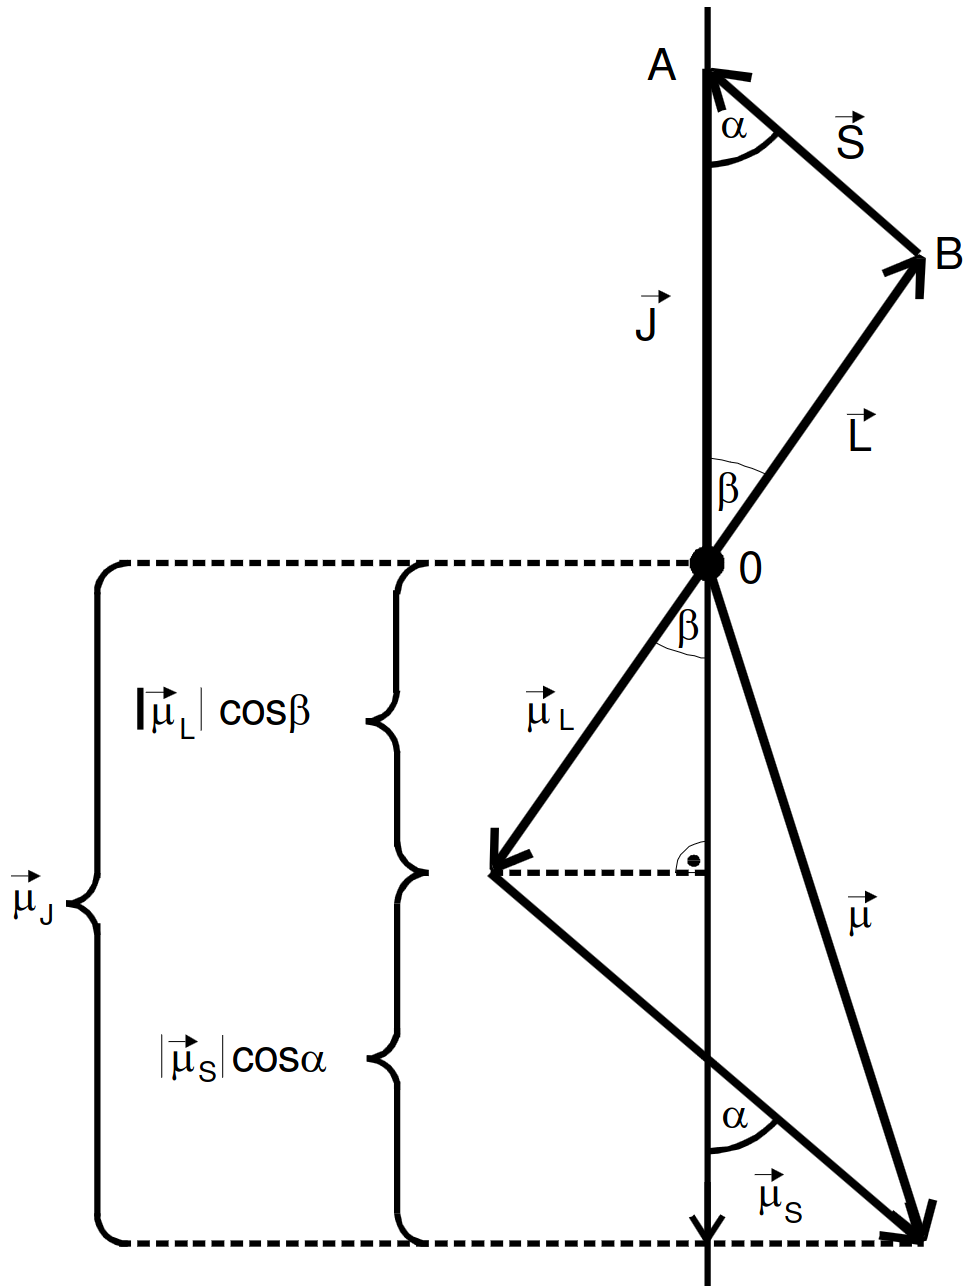
\includegraphics[width=0.6\textwidth]{img/LSKopplung.png}
    \caption{Vektorielle Aufspaltung der Drehimpulsvektoren und magnetischer Momente bei LS-Kopplung. \cite{V606}}
    \label{fig:LSKopplung}
\end{figure}

Bei der LS-Koppelung kann nur die zu $\vec{J}$ antiparallele oder parallele Komponente $\vec{μ}_J$ des magnetischen Moments gemessen werden.
Mit
\begin{equation*}
    |\vec{μ}_J| = |\vec{μ}_S| \cos(α) + |\vec{μ}_L| \cos(β)
\end{equation*}
kann das magnetische Moment berechnet werden.
Das Verhältnis der einzelnen Größen zueinander ist in \autoref{fig:LSKopplung} dargestellt.
Durch einsetzen der Beträge und geometrischen Überlegungen ergibt sich
\begin{equation*}
    |\vec{μ}_J| \approx μ_B g_J \sqrt{J(J+1)}
\end{equation*}
mit Landé-Faktor
\begin{equation*}
    g_J = \frac{3J(J+1) + S(S+1) - L(L+1)}{2J(J+1)}.
\end{equation*}
Hierbei ist $L$ die Bahndrehimpulsquantenzahl, $S$ die Spinquantenzahl und $J$ die Gesamtdrehimpulsquantenzahl.
\\
\\
\subsection{Richtungsquantelung}

Ein für diesen Versuch wichtiger Effekt ist die Richtungsquantelung.
Die Richtungsquantelung besagt, dass der Winkel zwischen der Richtung des magnetischen Moments und der Richtung des äußeren Magnetfeldes nur diskrete Werte annehmen kann.
Die Komponente $μ_{J_Z}$ von $\vec{μ}_J$ in Richtung des Magnetfeldes kann nur ein ganzzahliges Vielfaches ovn $μ_B g_J$ sein.
\begin{equation*}
    μ_{J_Z} = - μ_B g_J m.
\end{equation*}
Die Größe $m$ ist die Orientierungsquantenzahl. 
Diese Zahl kann Werte zwischen $\pm J$ annehmen, da eine einzelne Vektorkomponente nie größer als der Betrag des Vektors sein kann.
Wird ein Energieniveau in $2J+1$ Unterniveaus aufgespalten, so wird dies als Zeeman-Effekt bezeichnet.
Jede Einstellrichtung korrespondiert direkt zu einer potentiellen Energie, die berechnet werden kann mit
\begin{equation*}
    E_m = - μ_{J} B = μ_B g_J m B.
\end{equation*}
\\
\\
Die Magnetisierung einer Probe lässt sich berechnen mit dem betrag der ausgerichteten magnetischen Momente 
multipliziert mit der Häufigkeit der Ausrichtung summiert über alle vorkommenden Orientierungsquantenzahlen.
Über die Boltzmann-Verteilung $Z(E,T) = \exp(-\frac{E}{kT})$ ist die Besetzungsverteilung der Energieniveaus gegeben.
Das gesamte magnetische Moment der Probe ist dann
\begin{equation*}
    μ_{\text{ges}} = -μ_B g_J \sum_{m=-J}^{J} m \exp(-\frac{μ_B g_J\, m B}{kT}).
\end{equation*}
Teil man durch die Häufigkeit aller Ausrichtungen lässt sich das mittlere magnetische Moment berechnen
\begin{equation*}
    \bar{μ} = μ_B g_J \frac{\sum_{m=-J}^{J} m \exp(-\frac{μ_B g_J m B}{kT})}{\sum_{m=-J}^{J} \exp(-\frac{μ_B g_J m B}{kT})}.
\end{equation*}
Der verwendete Bruch wird als Brillouin-Funktion bezeichnet.
Der Betrag der Magnetisierung ist dann
\begin{equation}\label{eqn:M}
    M = μ_0 N \bar{μ}.
\end{equation}
Durch anwenden der Näherung
\begin{equation*}
    \frac{μ_B g_J m B}{kT} \ll 1
\end{equation*}
wird \autoref{eqn:M} zu
\begin{equation*}
    M = \frac{1}{3}μ_0 μ_B^2 g_J^2 N \frac{J(J + 1)B}{kT}.
\end{equation*}
Durch einsetzen in \autoref{eqn:Magnetisierung} und umstellen nach $χ$ ergibt sich
\begin{equation}\label{eqn:chi}
    χ = \frac{μ_0 μ_B^2 g_J^2 N J(J+1)}{3kT},
\end{equation}
wodurch gezeigt wird, dass die Suszeptibilität $χ ~ \frac{1}{T}$ Temperaturabhänig ist.
Dieser Umstand ist auch bekannt als Curiesches Gesetz des Paramagnetismus.

\subsection{Berechnung der Suszeptibilität von Seltenen Erden}

Verbindungen Seltener Erden zeigen starken Paramagnetismus. 
Dies lässt auf einen großen Drehimpuls der Elektronenhülle schließen.
Da auch Ionen Seltener Erden stark Paramagnetisch sind, muss das Phänomen auf innere Elektronen zurückführbar sein.
Bei allen Elementen der Seltenen Erden ist die gesamte Xenon-Elektronenhülle besetzt, sowie zwei 6s Elektronen.
Der Drehimpuls voll besetzter Orbitale ist Null, weshalb die 4f Elektronen für den Paramagnetismus verantwortlich sein müssen.
Da die 4f Elektronen innerhalb der 6s-Schale liegen, deckt sich die Überlegung mit der Beobachtung, dass auch die Ionen paramagnetisch sind.
\\
Das \textbf{Pauli-Prinzip} besagt, dass zwei Elektronen eines Atomes sich immer in mindestens einer Quantenzahl unterscheiden müssen.
Die konkrete Anordnung der Elektronen auf der 4f-Schale wird durch die \textbf{Hundschen Regeln} beschrieben:
\begin{enumerate}
    \item Die Spins der Elektronen auf einer Schale addieren sich zum maximalen Gesamtspin. Dies geschieht unter Beachtung des Pauli-Prinzips.
    \item Die Bahndrehimpulse addieren sich zum maximalen Gesamtbahndrehimpuls. Es muss das Pauli-Prinzip beachtet und Regel 1 erfüllt werden.
    \item Der Gesamtspin und der Gesamtbahndrehimpuls werden subtrahiert, um den Gesamtdrehimpuls zu erhalten falls die Schale weniger als halb voll besetzt ist. Der Gesamtspin und der Gesamtbahndrehimpuls werden addiert, um den Gesamtdrehimpuls zu erhalten falls die Schale mehr als halb voll besetzt ist.
\end{enumerate}
Zur Berechnung wird der Drehimpuls $\vec{J}$ und der Landé-Faktor $g_J$ benötigt.

\subsection{Messaparatur zur Messung der Suszeptibilität}

\begin{figure}[H]
    \centering
    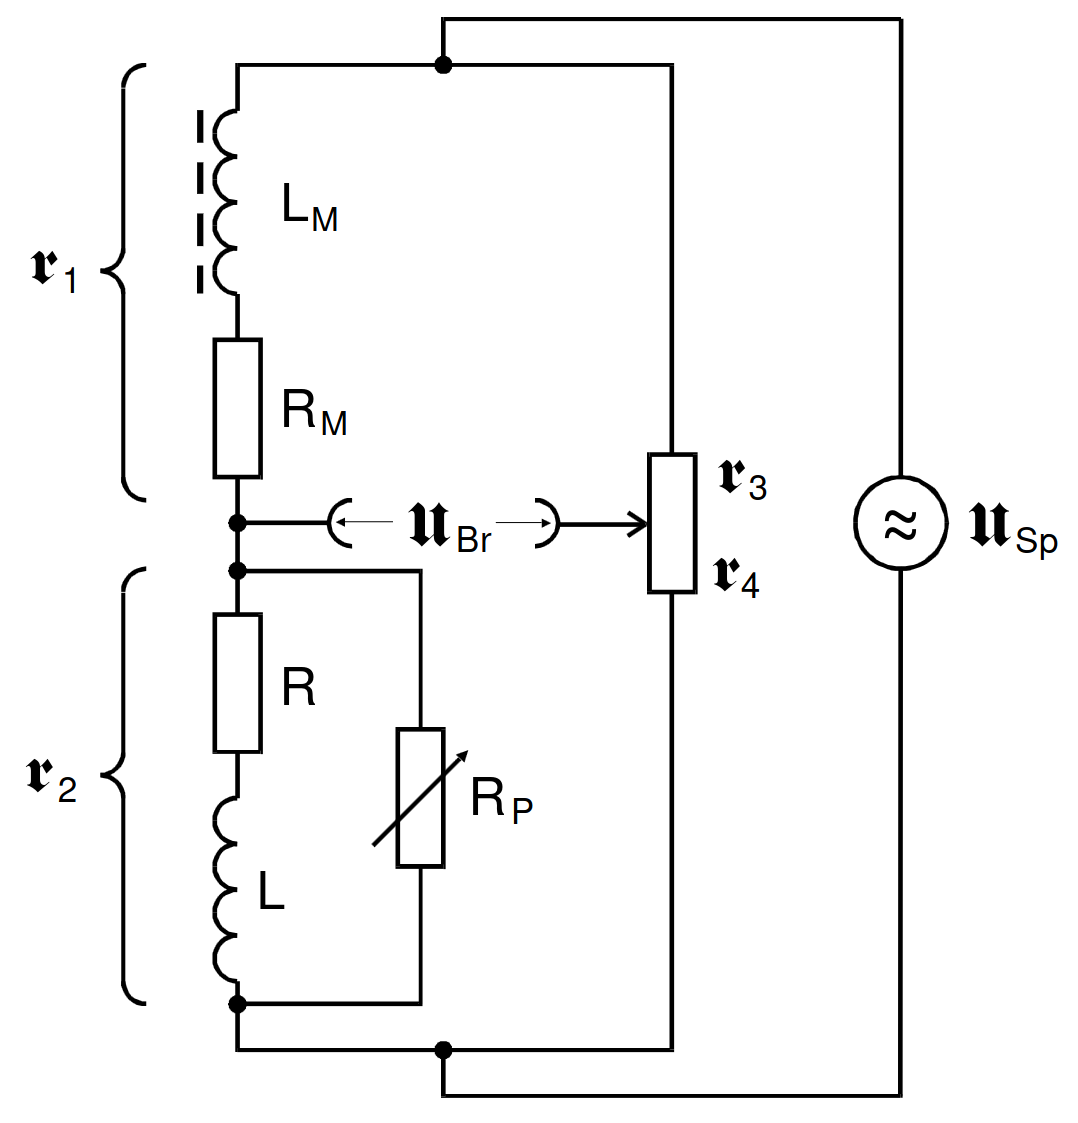
\includegraphics[width=0.7\textwidth]{img/bruecke.png}
    \caption{Schaltbild einer Brückenschaltung zur Messung der Suszeptibilität. \cite{V606}}
    \label{fig:bruecke}
\end{figure}

Um die Suszeptibilität von Seltenen Erden zu messen, wird die Veränderung der Induktivität einer Spule
durch die Probe gemessen.

Die Induktiviät einer langen Zylinderspule mit $N$ Windungen und Querschnittsfläche $F$ ist
\begin{equation}\label{eqn:L}
    L = μ_0 \frac{N^2 F}{l}.
\end{equation}
Durch einbringen einer Probe mit Querschnitt $Q$ wird die Induktivität zu
\begin{equation*}
    L_m = μ_0 \frac{N^2 F}{l} + χ μ_0 \frac{N^2 Q}{l}.
\end{equation*}
Die Differenz der Induktivitäten ist
\begin{equation}\label{eqn:deltaL}
    ΔL = χ μ_0 \frac{N^2 Q}{l}.
\end{equation}
Da $ΔL$ sehr klein ist, muss die Messung der Induktivität eine hohe Genauigkeit haben.
Dazu wird eine Brückenschaltung verwendet, die in \autoref{fig:bruecke} dargestellt ist.
Zur Messung der Induktivitätsdifferenz wird die Brücke auf ein Minimum abgeglichen.
Nach dem Einschieben der Probe wird die Brücke erneut abgeglichen.
Die Differenz des Widerstandes wird zur Berechnung der Induktivitätsdifferenz verwendet.%oder fur chi?
\\
\\
Für weitere Berechnungen wird die Brückenspannung benötigt, die entsteht wenn in die Spule $L_M$ die Probe eingeschoben wird.
Die Brückenspannung ist
\begin{equation}\label{eqn:Ubr}
    \mathfrak{U}_{\text{Br}} = \frac{\mathfrak{r}_4\mathfrak{r}_1 - \mathfrak{r}_3\mathfrak{r}_2}{(\mathfrak{r}_1 + \mathfrak{r}_2)(\mathfrak{r}_3 + \mathfrak{r}_4)} \mathfrak{U}_{\text{Sp}}.
\end{equation}
mit 
\begin{align*}
    \mathfrak{r}_1 &= R_M + iωL_M \\
    \frac{1}{\mathfrak{r}_2} &= \frac{1}{R_P} + \frac{1}{R + jωL}\\
    \mathfrak{r}_3 &= R_3\\
    \mathfrak{r}_4 &= R_4.
\end{align*}
Die Widerstände $R$ und $R_M$ sind dabei die Widerstände der Spulen. Sie sollten möglichst gleich sein.
Durch den Regelwiderstand $R_P$ werden die Beiden Wiederstände ausgeglichen. 
Es wird die Näherung $R_P >> R$ und $R_P >> ωL$ verwendet. Daraus folgt
\begin{equation*}
    \mathfrak{r}_2 \approx R + jωL.
\end{equation*}
Die beiden Widerstände $R_3$ und $R_4$ reell und etwa gleich groß.
Durch einsetzen der Widerstände mit den Näherungen ergibt sich
%\begin{equation*}
%    \mathfrak{U}_{\text{Br}} \approx \frac{1}{2} \frac{R_M - R + jω(L_M - L)}{R_M + R + jω(L_M + L)} \mathfrak{U}_{\text{Sp}}.
%\end{equation*}
\begin{equation*}
    \mathfrak{U}_{\text{Br}} \approx \frac{1}{2} \frac{jω(L_M - L)}{2R + jω(L_M + L)} \mathfrak{U}_{\text{Sp}}.
\end{equation*}
Die untersuchten Proben haben eine sehr kleine Suszeptibilität, weshalb $L_M = L$ mit $ΔL << L$ angenommen werden kann.
Daraus folgt
\begin{equation*}
    \mathfrak{U}_{\text{Br}} \approx \frac{ωΔL}{4}\frac{ωL + JR}{R^2 + ω^2L^2} \mathfrak{U}_{\text{Sp}}.
\end{equation*}
Durch Einsetzen der Werte für $L$ und $ΔL$ aus \eqref{eqn:L} und \eqref{eqn:deltaL} ergibt für den Betrag der Brückenspannung
\begin{equation*}
    U_{\text{Br}} = \frac{ωμ_0χN^2Q}{4l} \frac{1}{\sqrt{R^2 + ω^2\left(μ_0\frac{N^2}{l}F\right)^2}}.
\end{equation*}
So wird ein direkter Bezug zwischen der Brückenspannung und der Suszeptibilität hergestellt.
Für hohe Frequenzen $ω^2L^2 >> R^2$ lässt sich die nach $χ$ umgestellte Gleichung vereinfachen zu
\begin{equation}\label{eqn:chi2}
    χ = \frac{4F}{Q} \frac{U_{\text{Br}}}{U_{\text{Sp}}}.
\end{equation}
\\
\\
%Um chi explizit zu berechnen wird 
Um die Abgleichbedingung mit Probe zu berechnen wird zunächst die Abgleichsbedinung ohne Probe berechnet.
Aus \eqref{eqn:Ubr} folgt, dass
\begin{equation*}
    \mathfrak{r}_1R4 = \mathfrak{r}_2R_3.
\end{equation*}
Bevor die Probe eingeschoben wird, soll $R_3 \approx R_4$ gelten.
Um die Brückenspannung wieder zu minimieren nach Einbau der Probe wird $R_3$ angepasst
\begin{equation*}
    R_3' = R_3 + ΔR.
\end{equation*}
Da $R_3 + R_4 = const$ gilt, folgt für $R_4'$
\begin{equation*}
    R_4' = R_4 - ΔR \approx R_3 - ΔR.
\end{equation*}
Die Abgleichbedingung lautet dann
\begin{equation}\label{eqn:AbleichIm}
    (R_M + iωL_M)(R_3 + ΔR) = (R + iωL)(R_3 - ΔR).
\end{equation}
Der Imaginärteil der Gleichung \eqref{eqn:AbleichIm} kann zu 
\begin{equation}
    ΔR = \frac{R_3(L_M - L)}{L_M + L}
\end{equation}
umgeformt werden. Mit $ΔL << L$ kann die Gleichung vereinfacht werden zu
\begin{equation*}
    ΔR \approx \frac{ΔLR_3}{2L}.
\end{equation*}
Durch einsetzen für die Induktivität aus \eqref{eqn:L} und \eqref{eqn:deltaL} ergibt sich für die Widerstandsdifferenz
\begin{equation*}
    ΔR = χ\frac{R_3}{2} \frac{Q}{F}
\end{equation*}
und umgestellt nach $χ$ folgt
\begin{equation}\label{eqn:chi3}
    χ = \frac{2ΔR}{R_3} \frac{F}{Q}.
\end{equation}
\\
\\
\subsection{Unterdrückung der Störspannungen}

\begin{figure}[H]
    \centering
    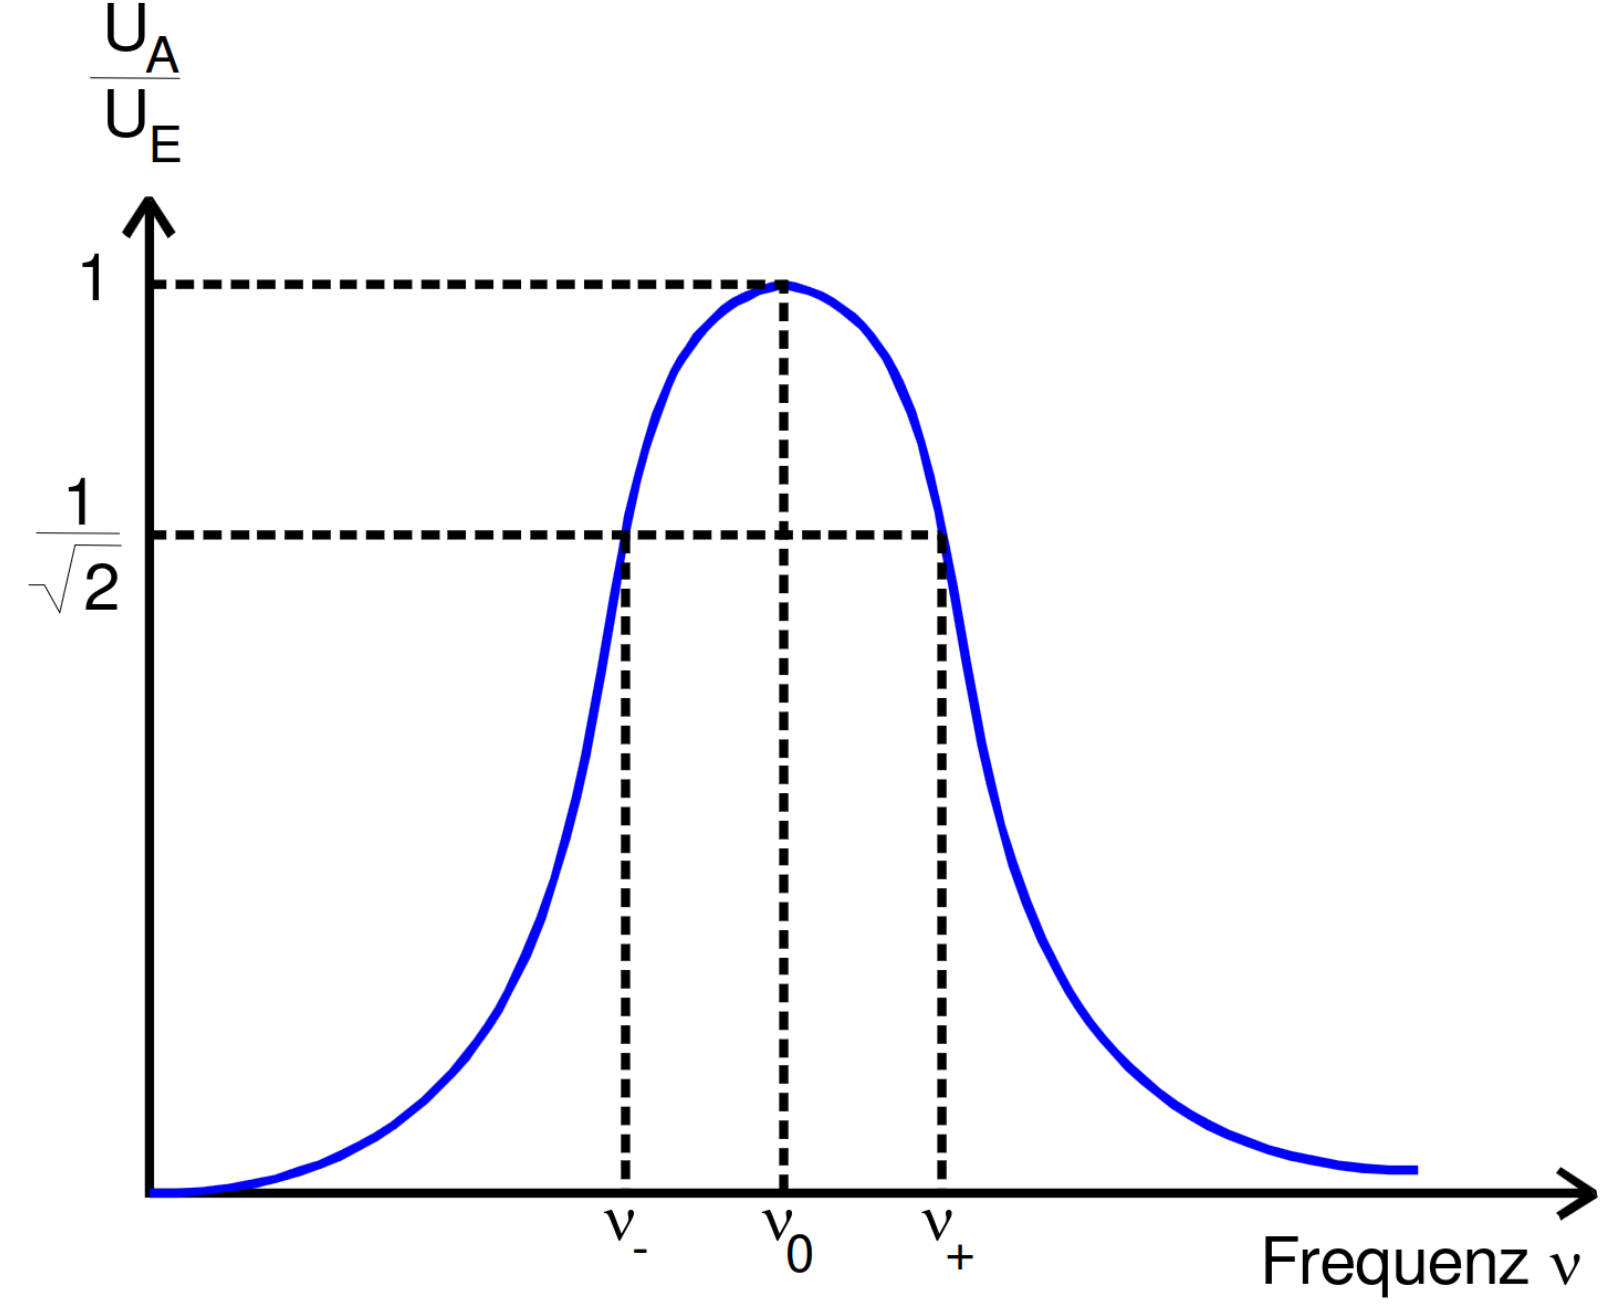
\includegraphics[width=0.7\textwidth]{img/Filterkurve.png}
    \caption{Verhältnis der Ausgangsspannung $U_A$ zur Eingangsspannung $U_E$ aufgetragen gegen die Frequenz\cite{V606}.}
    \label{fig:Filterkurve}
\end{figure}

Die Brückenspannung ist sehr viel geringer als die vorhandene Störspannung. 
Um diese zu unterdrücken wird ein Selektivverstärker verwendet.
Da die Signalspannung monofrequent ist, kann diese bei richtiger Frequenzwahl durch den Selektivversterkärker passieren.
Die Filterkurve in Abbildung \ref{fig:Filterkurve} zeigt, welche Frequenz eine Eingangsspannung besitzen muss nicht gefiltert zu werden.
Die Güte $Q$ ist ein Maß für die Breite der Filterkurve. Je höher die Güte, desto schmaler ist die Filterkurve.
Die Frequenz $f_0$ gibt das Maximum der Filterkurve an. Die Frequenzen $f_-$ und $f_+$ geben die Frequenzen an, bei denen die Ausgangsspannung auf $\frac{1}{\sqrt{2}}$ abgefallen ist.
Die Güte $Q$ ist definiert als
\begin{equation}\label{eqn:gute}
    Q = \frac{f_0}{f_+ - f_-}.
\end{equation}
